\documentclass{article}
\usepackage{graphicx}
\usepackage{float}
\usepackage{booktabs}
\usepackage{siunitx}

\title{Lab 2: Getting started with Ohm's Law, KVL, KCL, and Multi-Meter
Measurements}
\author{Sean Balbale}
\date{September 9th, 2023}
\setlength{\parindent}{0in}

\begin{document}

\begin{titlepage}
	\begin{center}
		\vspace*{1in}

		\Huge
		\textbf{Lab 2}

		\LARGE
		Getting started with Ohm’s Law, KVL, KCL, and Multi-Meter Measurements

		\vspace{3 in}

		\textbf{Student Name:} Sean Balbale
		\\ \textbf{Instructor:} Dr. Iman Salama
		\\ \textbf{Lab Partner Name:} Krish Gupta
		\\ \textbf{Date:} September 9th, 2024

		\vfill


	\end{center}
\end{titlepage}

\newpage


\section{Introduction}
The lab had a few primary purposes: practicing Ohm’s law,
KVL (Kirchhoff's voltage law), and KCL (Kirchhoff's current law),
and learning how to use a Multimeter. The Keysight power supply
and digital multimeter were used in this lab, which taught a
necessary skillset for all electrical engineers.

\section{Results}


\subsection{A Very Simple DC Circuit}
\begin{figure}[H]
	\centering
	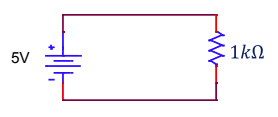
\includegraphics[width=0.5\textwidth]{simple_resistor_circuit_for_part1.png}
	\caption{Simple resistor circuit}
	\label{fig:fig1}
\end{figure}

During this lab section, a very simple circuit (Figure~\ref{fig:fig1}) was built on a
breadboard.

\begin{figure}[H]
	\centering
	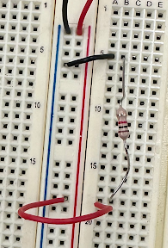
\includegraphics[angle=90,origin=c,width=0.5\textwidth]{built_figure1.png}
	\caption{Simple resistor circuit built on breadboard. The red wire is +5V while the black wire is ground.}
	\label{fig:fig2}
\end{figure}

Figure~\ref{fig:fig2} shows the circuit that was built.
The theoretical amperage flowing through the resistor can be calculated
using Ohm's Law. This calculation is shown in Equation (1).

\begin{equation}
	I = \frac{V}{R}
	\text{, where } V = 5V \text{ and } R = 1k\Omega
\end{equation}

The actual value of the resistor used was found to be $1.0004 \: k\Omega$. When
connected to a multimeter the voltage drop was measured to be $4.9986 \: V$.
The loop current was measured to be $4.9942 \: mA$. The measured values were close to the
calculated values, which is expected due to the accuracy of the equipment used.
The discrepancy between the calculated and measured values can be attributed to the
tolerance of the resistor and the accuracy of the multimeter. If the voltage over the
resistor doubles then, so will the loop current.

\subsection{KCL}
\begin{figure}[H]
	\centering
	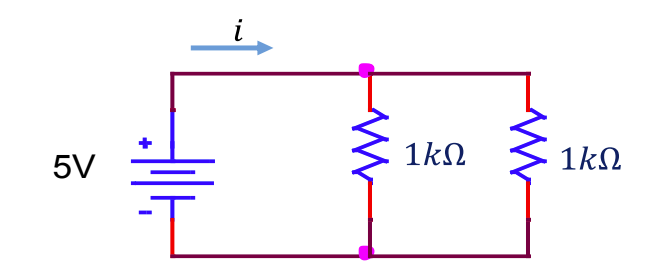
\includegraphics[width=0.5\textwidth]{parallel_resistor_for_part2.png}
	\caption{Parallel resistor circuit}
	\label{fig:fig3}
\end{figure}

During this lab section, a parallel resistor circuit (Figure~\ref{fig:fig3}) was built
on a breadboard.

\begin{figure}[H]
	\centering
	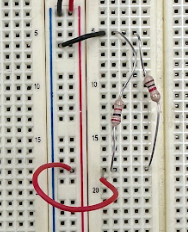
\includegraphics[angle=90,origin=c,width=0.5\textwidth]{built_figure3.png}
	\caption{Parallel resistor circuit built on breadboard. The red wire is +5V while the black wire is ground.}
	\label{fig:fig4}
\end{figure}

Figure~\ref{fig:fig4} shows the circuit that was built.
The theoretical amperage flowing through each resistor can be calculated
using KCL. This calculation is shown in Equation (2).

\begin{equation}
    I_{total} = I_1 + I_2 = \frac{V}{R_1} + \frac{V}{R_2}  
\end{equation}

After plugging in the values, the theoretical current through each resistor was
calculated to be $5 \: mA$ each.

The actual value of the resistors was found to be:
\begin{table}[H]
    \centering
    \begin{tabular}{|c|c|}
        \hline
        Resistor & Value $(k\Omega)$ \\
        \hline
        $R_1$ & 1.0002 \\
        \hline
        $R_2$ & 0.98635 \\
        \hline
    \end{tabular}
    \caption{Values of $R_1$ and $R_2$}
    \label{tab:2.2resistor_values}
\end{table}

After measuring the current through each resistor using the digital multimeter, 
the values were found to be:

\begin{table}[H]
    \centering
    \begin{tabular}{|c|c|}
        \hline
        Resistor & Value $(mA)$ \\
        \hline
        $R_1$ & 4.9938 \\
        \hline
        $R_2$ & 5.06119 \\
        \hline
        $Total$ & 10.0501 \\
        \hline
    \end{tabular}
    \caption{Current Running Through $R_1$ and $R_2$}
    \label{tab:2.3resistor_currents}
\end{table}

These measured values were close to the calculated values, which is expected 
due to the accuracy of the equipment used. They also satisfy KCL, as the total
current through the circuit is equal to the sum of the currents through each resistor.
\newline

After changing $R_1$ to $2k\Omega$, which was measured to be $1.9419k\Omega$. The current through 
$R_1$ was measured to be $2.5714mA$ and the current through $R_2$ was measured to be $5.0671mA$. 
The total current was measured to be $7.6329mA$. These values also satisfy KCL.

\subsection{KVL}
\begin{figure}[H]
	\centering
	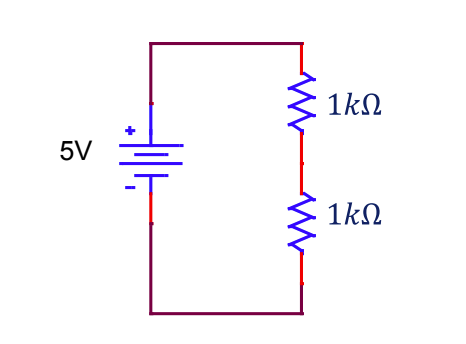
\includegraphics[width=0.5\textwidth]{series_resistor_circuit_for_part3.png}
	\caption{Series resistor circuit}
	\label{fig:fig5}
\end{figure}

During this lab section, a series resistor circuit (Figure~\ref{fig:fig5}) was built
on a breadboard.

\begin{figure}[H]
	\centering
	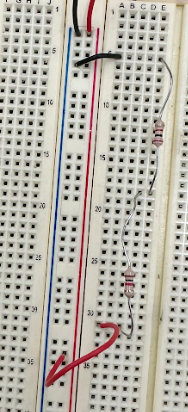
\includegraphics[angle=90,origin=c,width=0.5\textwidth]{built_figure5.png}
	\caption{Series resistor circuit built on breadboard. The red wire is +5V while the black wire is ground.}
	\label{fig:fig6}
\end{figure}

Figure~\ref{fig:fig6} shows the circuit that was built.
The theoretical voltages across each resistor can be calculated using KVL. 
This calculation is shown in Equation (3).

\begin{equation}
    V_{total} = V_1 + V_2
\end{equation}

After plugging in the values, the theoretical voltage across each resistor was
calculated to be $2.5 \: V$ each.

The actual value of the resistors was found to be:
\begin{table}[H]
    \centering
    \begin{tabular}{|c|c|}
        \hline
        Resistor & Value $(k\Omega)$ \\
        \hline
        $R_1$ & 0.98601 \\
        \hline
        $R_2$ & 0.99970 \\
        \hline
    \end{tabular}
    \caption{Values of $R_1$ and $R_2$}
    \label{tab:2.4resistor_values}
\end{table}
 The voltages measured across the resistors were found to be:
\begin{table}[H]
    \centering
    \begin{tabular}{|c|c|}
        \hline
        Resistor & Value $(V)$ \\
        \hline
        $R_1$ & 2.4822 \\
        \hline
        $R_2$ & 2.5172 \\
        \hline
        $Total$ & 4.9995 \\
        \hline
    \end{tabular}
    \caption{Voltage Across $R_1$ and $R_2$}
    \label{tab:2.5resistor_voltages}
\end{table}

The results were close to the calculated values, which is expected due 
to the accuracy of the equipment used. They also satisfy KVL, as the total 
voltage across the circuit is equal to the sum of the voltages across each resistor.
\newline

After changing $R_1$ to $2k\Omega$, which was measured to be $1.9420 k\Omega$. The voltage across
$R_1$ was measured to be $3.3004V$ and the voltage across $R_2$ was measured to be $1.6990V$. 
These values also satisfy KVL. Finally, if the two resistors are disconnected from the circuit.

\begin{figure}[H]
	\centering
	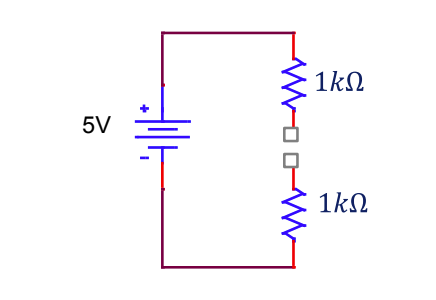
\includegraphics[width=0.5\textwidth]{disconnected_(open)_circuit.png}
	\caption{Disconnected (open) circuit}
	\label{fig:fig7}
\end{figure}

The voltage across the open circuit was measured to be $4.9995V$. The ammount of current 
flowing through the circuit was $5.000mA$. This measurement implies that the multimeter has 
a very high resistance, which is why the voltage across the open circuit is the same as the
voltage across the circuit with the resistors. In addition, the current flowing through the
circuit is the same as the current flowing through the circuit with the resistors.

\section{Discussions and Conclusions}

In this lab, we successfully verified Ohm's Law and 
Kirchhoff's Voltage Law (KVL) through practical measurements 
and calculations. The measured voltages across resistors $R_1$ 
and $R_2$ were consistent with the theoretical values, demonstrating 
the accuracy of our equipment and the validity of the laws in a 
real-world scenario.
\newline

When $R_1$ was changed to $2k\Omega$ (measured as $1.9420 k\Omega$), 
the measured voltages across $R_1$ and $R_2$ were $3.3004V$ 
and $1.6990V$ respectively. These values also satisfied KVL, 
further confirming the reliability of our measurements and the 
theoretical principles.
\newline

Additionally, the voltage across the open circuit was measured 
to be $4.9995V$, and the current flowing through the circuit was 
$5.000mA$. These measurements indicate that the multimeter used has a 
very high internal resistance, which explains why the voltage across 
the open circuit remained the same as when the resistors were connected.
\newline

Overall, the experiment demonstrated the fundamental principles 
of Ohm's Law and KVL, and highlighted the importance of accurate 
measurements in electrical circuit analysis. The results obtained 
were in close agreement with the theoretical predictions, validating 
the experimental setup and the procedures followed.

\section{References}
 [1] Dr. Iman Salama. “Lab 2 – Getting started with Ohm’s Law, KVL, KCL,
and Multi-Meter Measurements” Northeastern University. 9 September 2024.

\end{document}
